% SPDX-License-Identifier: CC-BY-4.0
% DBOR specification - Dense Binary Object Representation
% Copyright (C) 2020 Daniel Lutz <dlu-ch@users.noreply.github.com>

\documentclass{dbor-article}

    \pdfsuppresswarningpagegroup=1

    % mathematical symbols and operators
    \newcommand{\e}{\mathrm{e}}
    \DeclareMathOperator{\BitAnd}{AND}
    \DeclareMathOperator{\BitOr}{OR}
    \newcommand{\SetOfIntegers}{\mathbbm{Z}}
    \newcommand{\BinNumber}[1]{\mathrm{#1}_{2}}
    \newcommand{\HexNumber}[1]{\mathrm{#1}_{16}}
    \newcommand{\IntegerInterval}[2]{\{#1 \,\ldots\, #2\}}

    \newcommand{\Concat}{\ensuremath{\lrtimes}}

    \newcommand{\ByteSequence}[1]{\ensuremath{\langle #1 \rangle}}

    \newcommand{\DborSyntaxIdent}[1]{\texttt{#1}}
    \newcommand{\DborSyntaxIdentRef}[1]{\hyperlink{sec:def:#1}{\DborSyntaxIdent{#1}}}
        % usage: \DborSyntaxIdentRef{IntegerToken}

    % colour coding of bytes sequences
    \newcommand{\DborFirstByte}[2]{\textcolor{#1}{\ensuremath{\bm{\HexNumber{#2}}}}}
    \newcommand{\DborFirstByteNone}[1]{\DborFirstByte{red-std}{#1}}
    \newcommand{\DborFirstByteNumber}[1]{\DborFirstByte{black}{#1}}
        % IntegerValue, BinaryRationalValue, DecimalRationalValue, MinusZero, Infinity, MinusInfinity
    \newcommand{\DborFirstByteString}[1]{\DborFirstByte{green-std}{#1}}
        % ByteStringValue, Utf8StringValue
    \newcommand{\DborFirstByteSequence}[1]{\DborFirstByte{blue-std}{#1}}
    \newcommand{\DborFirstByteDictionary}[1]{\DborFirstByte{violet-std}{#1}}
    \newcommand{\DborFirstByteAllocated}[1]{\DborFirstByte{gray-std}{#1}}
    \newcommand{\DborNextByte}[1]{\ensuremath{\HexNumber{#1}}}
    \newcommand{\DborNextByteFill}[1]{\textcolor{gray-std}{\ensuremath{\HexNumber{#1}}}}

    \newenvironment{Note}{\medskip\bgroup\small\ignorespaces}{\par\egroup\smallskip}

    \newcommand{\IncludeImageInPlace}[1]{%
        \begin{quotation}%
            \noindent
            \includegraphics[scale=0.8]{#1}%
        \end{quotation}%
    }

    \newcommand{\DborVersion}{\input{repo_wd_version.tex}}
    \title{DBOR specification \DborVersion}
    \author{Daniel Lutz}

\begin{document}

    \maketitle
    \tableofcontents

    % SPDX-License-Identifier: CC-BY-4.0
% DBOR specification - Dense Binary Object Representation
% Copyright (C) 2020 Daniel Lutz <dlu-ch@users.noreply.github.com>

\section{Introduction}
%%%%%%%%%%%%%%%%%%%%%%

\subsection{Terms and definitions}
%%%%%%%%%%%%%%%%%%%%%%%%%%%%%%%%%%

In this specification, $N$ always denotes the constant $\sum_{i = 0}^8 2^{8i} \approx 1.003921 \cdot 2^{64}$.


\subsection{Notation}
%%%%%%%%%%%%%%%%%%%%%

\noindent
{%
    \setlength\extrarowheight{0.8ex}%
    \begin{tabular}{@{} p{.1\textwidth} p{.8\textwidth}}
        $\SetOfIntegers$: &
            the set of all real integers \\
        $\IntegerInterval{a}{b}$: &
            $\{i \in \SetOfIntegers{:}\; a \le i \le b\}$ \\
        $\ByteSequence{a, b, \ldots}$: &
            byte sequence, starting with byte $a$ \\
        $a \Concat b$: &
            concatenation of bytes sequences $a$, $b$: $a$ followed by $b$ \\
        $\|a\|$: &
            size of bytes sequence $a$ in byte
    \end{tabular}%
}

    % SPDX-License-Identifier: CC-BY-4.0
% DBOR specification - Dense Binary Object Representation
% Copyright (C) 2020 Daniel Lutz <dlu-ch@users.noreply.github.com>

\section{Values}
%%%%%%%%%%%%%%%%
\label{sec:values}

This section defines the representation of objects as bytes sequences - the core of DBOR.
A byte sequence that represents a single object is called \emph{value} and is composed of \emph{tokens}
(defined in section \ref{sec:tokens}).


\subsection{Overview (\DborValue)}
%%%%%%%%%%%%%%%%%%%%%%%%%%%%%%%%%%
\hypertarget{sec:def:Value}{}

% Relation between value and byte sequence
DBOR represents a sequence of \emph{objects} $O^*$ as a concatenation $B^*$ of their \emph{representations as byte
sequences} in such a way that the efficient reconstruction of $O^*$ from $B^*$ alone is possible by traversing $B^*$
in forward direction:
\begin{align*}
    \text{objects} & \quad\rightarrow\quad \text{byte sequence} \\[-2ex]
    -100, \text{"¡Olé!"}
        & \quad\mapsto\quad
    \ByteSequence{
        \underbrace{%
            \DborFirstByteNumber{38}, \DborNextByte{4B}
        }_{\hskip-\textwidth\DborIntegerValue(-100)\hskip-\textwidth},
        %
        \overbrace{%
            \DborFirstByteString{67},
            \DborNextByte{C2}, \DborNextByte{A1},
            \DborNextByte{4F}, \DborNextByte{6C},
            \DborNextByte{C3}, \DborNextByte{A9},
            \DborNextByte{21}
        }^{\DborUtfEightStringValue(\text{"¡Olé!"})}
    }
\end{align*}
The representation is byte oriented and does not depend on word alignment or endianness.
The byte sequence of each encoded object contains its own size.

\medskip
DBOR \emph{focuses on the represented "value" of an object} to be encoded, not its type --
an unsigned $8$~bit number $42$ is no different from signed $64$~bit number $42$ in this view.%
\footnote{%
    This approach enables the definition and simple implementation of compatible interfaces between independent systems.

    Let's assume you need to send an unsigned $8$~bit number~$x$ as part of a command from a system~$A$ to
    an independent system~$B$ over a EIA-232 connection~$T$.
    \begin{enumerate}
        \item
        You implement the handling of $x$ as unsigned $8$~bit number on $A$ and $B$ and its transport over $T$
        as \DborIntegerValue{}.
        Then you release the systems~$A_1$ and $B_1$.

        \item
        You find out than $x$ sometimes needs $16$~bits.
        Therefore you adapt $A$ and $B$ to support this larger numbers and release $A_2$ and $B_2$.
    \end{enumerate}

    In the result, $A_1$ or $A_2$ can send the number $100$ to $B_1$ or $B_2$ and
    $A_2$ can send the number $1000$ to $B_1$ or $B_2$.
    When $B_2$ receives the number $1000$ from $A_2$, it rejects the command due to an argument larger than supported.
    All other combinations work as expected.

    The same applies when you replace an \DborIntegerValue{} by any other subclass of \DborNumberValue{}.
}
The byte sequence encoding an object is therefore called "value".
Wherever possible in a simple and efficient way, DBOR choses the shortest byte sequence to represent an object.

\medskip
DBOR groups objects of a common nature to be represented and encoded in a similar way by \emph{classes}
named \DborSyntaxIdent{}{\dots Value}.
The expression \DborIntegerValue($-100$) means the byte sequence that represents $-100$ as an instance of
class \DborIntegerValue{}:
\begin{equation*}
    \begin{array}{c}
        \DborIntegerValue(-1) \\
        = \ByteSequence{\DborFirstByteNumber{38}, \DborNextByte{4B}}
    \end{array}
    \quad\text{is an instance of}\quad \DborIntegerValue
\end{equation*}
Each value comprises in its first byte of the (concrete) class that it is an instance of.

\medskip
An abstract class like \DborNumberValue{} represent common traits of objects and can be used as placeholder for any
of its concrete subclasses (like \DborIntegerValue{} or \DborInfinityValue{} in this case).
The byte sequence \ByteSequence{\DborFirstByteNumber{38}, \DborNextByte{4B}} "is a" \DborNumberValue{},
an \DborElementaryValue{}, and a \DborValue{} (all abstract classes).

\begin{figure}[H]
    \begin{quote}
        \noindent
        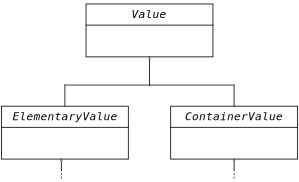
\includegraphics[scale=0.7]{classdiag_value}%
        \caption{Class hierarchy of values.}
        \label{fig:class:Value}
    \end{quote}
\end{figure}

See section~\ref{sec:elementaryvalues} and \ref{sec:containervalues} for a complete list of (concrete) values.


\subsection{Elementary values (\DborElementaryValue, \DborNumberValue, \DborStringValue)}
%%%%%%%%%%%%%%%%%%%%%%%%%%%%%%%%%%%%%%%%%%%%%%%%%%%%%%%%%%%%%%%%%%%%%%%%%%%%%%%%%%%%%%%%%
\label{sec:elementaryvalues}
\hypertarget{sec:def:ElementaryValue}{}
\hypertarget{sec:def:NumberValue}{}
\hypertarget{sec:def:StringValue}{}

Elementary values are values that represent a single object with a meaning of its own (e.g. an integer).

% TODO complete

\begin{figure}[H]
    \begin{quote}
        \noindent
        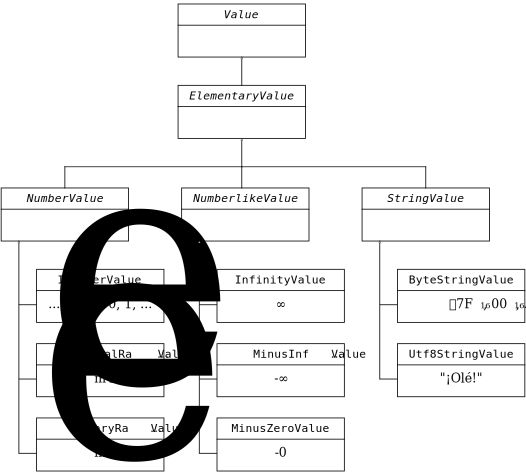
\includegraphics[scale=0.7]{classdiag_elementary}%
        \caption{Class hierarchy of elementary values.}
        \label{fig:class:ElementaryValue}
    \end{quote}
\end{figure}


\subsubsection{\DborNoneValue}
%%%%%%%%%%%%%%%%%%%%%%%%%%%%%%
\label{sec:def:NoneValue}
\hypertarget{sec:def:NoneValue}{}

\paragraph{Representable objects}

A \DborNoneValue{} represents the absence of an actual object (like \texttt{null} or \texttt{None} in some
programming languages or NaN in IEEE-754:2008).
It is considered different from any object represented by a \DborValue*{} other than \DborNoneValue.

\paragraph{Representation}

A \DborNoneValue{} is the \DborMinimalToken*($3$, $\HexNumber{1F}$).

\smallskip
\noindent
Example:\nolinebreak
\begin{quote}
    \noindent
    \begin{tabular}{ll}
        \toprule
        Value & Representation \\
        \midrule
        \DborNoneValue & \ByteSequence{\DborFirstByteNone{FF}} \\
        \bottomrule
    \end{tabular}
\end{quote}

\paragraph{Ambiguity, canonical value}

There is only one representation of a \DborNoneValue.
It is canonical.
Every \DborNoneValue{} is well-formed.


\subsubsection{\DborMinusZeroValue, \DborInfinityValue, \DborMinusInfinityValue}
%%%%%%%%%%%%%%%%%%%%%%%%%%%%%%%%%%%%%%%%%%%%%%%%%%%%%%%%%%%%%%%%%%%%%%%%%%%%%%%%
\label{sec:def:MinusZeroValue}
\label{sec:def:InfinityValue}
\label{sec:def:MinusInfinityValue}
\hypertarget{sec:def:MinusZeroValue}{}
\hypertarget{sec:def:InfinityValue}{}
\hypertarget{sec:def:MinusInfinityValue}{}

\paragraph{Representable objects}

A \DborMinusZeroValue{} represents the "number" $-0$ in the sense of IEEE-754:2008 arithmetic.

A \DborInfinityValue{} represents the "number" $\infty$ in the sense of IEEE-754:2008 arithmetic.
It is considered larger than any object represented by a \DborNumberValue*{}
other than \DborInfinityValue.

A \DborMinusInfinityValue{} represents the "number" $-\infty$ in the sense of IEEE-754:2008 arithmetic.
It is considered smaller than any object represented by a \DborNumberValue*{}
other than \DborMinusInfinityValue.

\paragraph{Representation}

A \DborMinusZeroValue{} is the \DborMinimalToken*($3$, $\HexNumber{1C}$).

An \DborInfinityValue{} is the \DborMinimalToken*($3$, $\HexNumber{1E}$).

A \DborMinusInfinityValue{} is the \DborMinimalToken*($3$, $\HexNumber{1D}$).

\smallskip
\noindent
Examples:\nolinebreak
\begin{quote}
    \noindent
    \begin{tabular}{ll}
        \toprule
        Value & Representation \\
        \midrule
        \DborMinusZeroValue & \ByteSequence{\DborFirstByteNumber{FC}} \\
        \DborInfinityValue & \ByteSequence{\DborFirstByteNumber{FE}} \\
        \DborMinusInfinityValue & \ByteSequence{\DborFirstByteNumber{FD}} \\
        \bottomrule
    \end{tabular}
\end{quote}

\paragraph{Ambiguity, canonical value}

There is only one representation of a \DborMinusZeroValue,
\DborInfinityValue, and \DborMinusInfinityValue, respectively.
They are canonical.
Every \DborMinusZeroValue, \DborInfinityValue,
and \DborMinusInfinityValue{} is well-formed.


\subsubsection{\DborIntegerValue($v$)}
%%%%%%%%%%%%%%%%%%%%%%%%%%%%%%%%%%%%%%%%%%%%%%%%%%%
\hypertarget{sec:def:IntegerValue}{}

\paragraph{Representable objects}

An \DborIntegerValue{} can represent any number $v \in \IntegerInterval{-(N + 24)}{N + 23}$.

\smallskip
The minimum representable number is $-18\,519\,084\,246\,547\,628\,312$.
The maximum representable number is $18\,519\,084\,246\,547\,628\,311$.

\paragraph{Representation}

A number $v \in \IntegerInterval{0}{N + 23}$ is represented as \DborIntegerToken*(0, $v$).
A number $v \in \IntegerInterval{-(N + 24)}{0}$ is represented as \DborIntegerToken*(1, $-v - 1$).

\smallskip
\noindent
Examples:\nolinebreak
\begin{quote}
    \noindent
    \begin{tabular}{ll}
        \toprule
        Value & Representation \\
        \midrule
        %
        \DborIntegerValue($0$)
            &  \ByteSequence{\DborFirstByteNumber{00}} \\
        \DborIntegerValue($-1$)
            &  \ByteSequence{\DborFirstByteNumber{20}} \\
        \DborIntegerValue($23$)
            &  \ByteSequence{\DborFirstByteNumber{17}} \\
        \DborIntegerValue($24$)
            &  \ByteSequence{\DborFirstByteNumber{18}, \DborNextByte{00}} \\
        \DborIntegerValue($-100$)
            &  \ByteSequence{\DborFirstByteNumber{38}, \DborNextByte{4B}} \\
        \DborIntegerValue($\HexNumber{FF\,FF\,FF\,FF}$)
            &  \ByteSequence{\DborFirstByteNumber{1B}, \DborNextByte{E7}, \DborNextByte{FE},
               \DborNextByte{FE}, \DborNextByte{FE}} \\
        %
        \bottomrule
    \end{tabular}
\end{quote}

A non-empty byte sequence \ByteSequence{b_1, \ldots, b_n} is a \emph{well-formed} \DborIntegerValue{}
if and only if it is an \DborIntegerToken*(0, $w$) or an \DborIntegerToken*(1, $w$) for
an appropriate $w$.
The sequence is an \emph{ill-formed} \DborIntegerValue{} if and only if it is not a well-formed
\DborIntegerValue{} but $b_1$ is the first byte of a \DborIntegerToken*(0, $w$) or
an \DborIntegerToken*(1, $w$).

\paragraph{Ambiguity, canonical value}

There is at most one representation of a \DborIntegerValue($v$) for any $v$.
It is canonical.


\subsubsection{\DborBinaryRationalValue($p$, $v$)}
%%%%%%%%%%%%%%%%%%%%%%%%%%%%%%%%%%%%%%%%%%%%%%%%%%%%%
\hypertarget{sec:def:BinaryRationalValue}{}

\paragraph{Representable objects}

A \DborBinaryRationalValue can represent any number
\begin{equation}
    v = (-1)^s \cdot \sum_{i = -52}^0 m_i s^i \cdot 2^e
\end{equation}
with $s, m_i \in \{0, 1\}$, $e \in \IntegerInterval{2 - 2^{10}}{2^{10}}$ and $v \ne 0$.

The set of representable numbers comprises all normal and subnormal values of the IEEE-754:2008 type
\texttt{binary64} except $\pm 0$.

\smallskip
The maximum representable number is $(2 - 2^{-52}) \cdot 2^{2^{10}} \approx 3.595\,386 \cdot 10^{308}$.
The smallest positive representable number is $2^{-52} \cdot 2^{2-2^{10}} = 2^{-1074}
\approx 4.940\,656 \cdot 10^{-324}$.

\paragraph{Representation}

A number $(-1)^s \cdot (1 + M/2^p) \cdot 2^e$ with
\begin{align*}
    s & \in \{0, 1\} \\
    p & \in \{4, 10, 16, 23, 30, 37, 44, 52\} \\
    M & \in \IntegerInterval{0}{2^p - 1} \\
    e & \in \IntegerInterval{\max(0, p - 51) - 2^{r - 1} + 1}{2^{r - 1} - 1} \\
    r & := 8 \lfloor p / 7 \rfloor + 7 - p
\end{align*}%
is represented as
\DborBinaryRationalToken*($p$, $0$, $s$, $M$, $e + 2^{r - 1} - 1$).

A number $(-1)^s \cdot M/2^p \cdot 2^{-1022}$ with $p := 52$, $s \in \{0, 1\}$ and
$M \in \SetOfIntegers \cap (0, 2^p)$ is represented as
\DborBinaryRationalToken*($p$, $1$, $s$, $M$, $0$).

\smallskip
\noindent
For reference, here are the resulting combinations for all possible $p$:\nolinebreak
\begin{quote}
    \newcolumntype{R}{>{$}r<{$}}  % package 'array'
    \begin{tabular}{R R R R >{\hspace{-.8em}$}c<{$\hspace{-.8em}} R}
        \toprule
        k & p & r & & e \\
        \midrule
        0 &  3 &  4 & -3 & \ldots & 4 \\
        1 &  5 & 10 & -15 & \ldots & 16 \\
        2 &  7 & 16 & -63 & \ldots & 64 \\
        3 &  8 & 23 & -127 & \ldots & 128 \\
        4 &  9 & 30 & -255 & \ldots & 256 \\
        5 & 10 & 37 & -511 & \ldots & 512 \\
        6 & 11 & 44 & -1023 & \ldots & 1024 \\
        7 & 11 & 52 & -1022 & \ldots & 1024 \\
        \bottomrule
    \end{tabular}
\end{quote}

\smallskip
\noindent
Examples:\nolinebreak
\begin{quote}
    \noindent
    \begin{tabular}{ll}
        \toprule
        Value & Representation \\
        \midrule
        \DborBinaryRationalValue($3$, $\frac{1}{8}$)
            &  \ByteSequence{\DborFirstByteNumber{D0}, \DborNextByte{00}} \\
        \DborBinaryRationalValue($5$, $-(2^{17} - 2^6)$)%
            \footnote{$-\left(1 + (1 - 2^{-10})\right) \cdot 2^{16}$}
            &  \ByteSequence{\DborFirstByteNumber{D1}, \DborNextByte{FF}, \DborNextByte{FF}} \\
        \DborBinaryRationalValue($52$, $2^{-1074}$)
            &  $\ByteSequence{\DborFirstByteNumber{D7}, \DborNextByte{01}, \DborNextByte{00},
                                                        \DborNextByte{00}, \DborNextByte{00},$ \\
            &  $                                        \DborNextByte{00}, \DborNextByte{00},
                                                        \DborNextByte{00}, \DborNextByte{00}}$ \\
        \bottomrule
    \end{tabular}
\end{quote}

A non-empty byte sequence \ByteSequence{b_1, \ldots, b_n} is a \emph{well-formed}
\DborBinaryRationalValue{} if and only if
it is a \DborBinaryRationalToken*($p$, $o$, $s$, $M$, $E$) for some appropriate $p$, $o$, $s$, $M$ and $E$.
The sequence is an \emph{ill-formed} \DborBinaryRationalValue{} if and only if it is not a well-formed
\DborBinaryRationalValue{} but $b_1$ is the first byte of a
\DborBinaryRationalToken*($p$, $o$, $s$, $M$, $E$).

\paragraph{Ambiguity, canonical value}

There may be more than one representation of \DborBinaryRationalValue($p$, $v$) for any $v$.
Of these, the one with the smallest $p$ is the canonical value.%
\footnote{
    A \DborBinaryRationalValue($p$, $v$) is therefore canonical if and only if there is
    no \DborBinaryRationalValue($q$, $v$) with $q < p$.
    See \ref{sec:implementation:BinaryRationalValue:canonical} for an efficient way to check this.
}

For every \DborBinaryRationalValue($p$, $v$) with $p < 52$, there is also
a \DborBinaryRationalValue($p$, $v$) for any
$q \in \{4, 10, 16, 23, 30, 37, 44, 52\}$ with $q > p$.


\subsubsection{\DborDecimalRationalValue($m$, $e$)}
%%%%%%%%%%%%%%%%%%%%%%%%%%%%%%%%%%%%%%%%%%%%%%%%%%%
\hypertarget{sec:def:DecimalRationalValue}{}

\paragraph{Representable objects}

A \DborDecimalRationalValue{} can represent any number
\begin{equation}
    v = m \cdot 10^e
\end{equation}
with
\begin{align*}
    m & \in \IntegerInterval{-(N + 24)}{-1} \cup \IntegerInterval{1}{N + 23} \\
    e & \in \IntegerInterval{-(N + 8)}{-1} \cup \IntegerInterval{1}{N + 8}
\end{align*}

\smallskip
The minimum representable number is $-18\,519\,084\,246\,547\,628\,312 \cdot 10^{18\,519\,084\,246\,547\,628\,296}$.
The maximum representable number is $18\,519\,084\,246\,547\,628\,311 \cdot 10^{18\,519\,084\,246\,547\,628\,296}$.
The smallest positive representable number is $10^{-18\,519\,084\,246\,547\,628\,296}$.

\paragraph{Representation}

A number $m \cdot 10^e$ with with $m \in \IntegerInterval{-(N + 24)}{-1} \cup \IntegerInterval{1}{N + 23}$
and $e \in \IntegerInterval{-(N + 8)}{-1} \cup \IntegerInterval{1}{N + 8}$
is represented as \DborPowerOfTenToken*($e$) {\Concat} \DborIntegerValue*($m$).

\smallskip
\noindent
Examples:\nolinebreak
\begin{quote}
    \noindent
    \begin{tabular}{ll}
        \toprule
        Value & Representation \\
        \midrule
        \DborDecimalRationalValue($1$, $-2$)
            &  \ByteSequence{\DborFirstByteNumber{E9}, \DborNextByte{01}} \\
        \DborDecimalRationalValue($-123$, $100$)
            &  \ByteSequence{\DborFirstByteNumber{C0}, \DborNextByte{5B}, \DborNextByte{38}, \DborNextByte{62}} \\
        \bottomrule
    \end{tabular}
\end{quote}

A non-empty byte sequence \ByteSequence{b_1, \ldots, b_n} is a \emph{well-formed}
\DborDecimalRationalValue{} if and only if
it is \DborPowerOfTenToken*($e$) {\Concat} \DborIntegerToken*($m$) for
appropriate $m \ne 0$ and $e$.
The sequence is an \emph{ill-formed} \DborDecimalRationalValue{} if and only if it is not a well-formed
\DborDecimalRationalValue{} but $b_1$ is the first byte of a \DborPowerOfTenToken*($e$).

\paragraph{Ambiguity, canonical value}

There may be more than one \DborDecimalRationalValue($m$, $e$) representing the same number $m \cdot 10^e$.
Of these, the one with the smallest $|m|$ is the canonical value.%
\footnote{
    A \DborDecimalRationalValue($m$, $e$) is therefore canonical if and only if $m \bmod 10 = 0$.
    See \ref{sec:implementation:IntegerValue:mod10} for an efficient way to check this.
}


\subsubsection{\DborByteStringValue(\ByteSequence{b_1, \ldots, b_m})}
%%%%%%%%%%%%%%%%%%%%%%%%%%%%%%%%%%%%%%%%%%%%%%%%%%%%%%%%%%%%%%%%%%%%%
\hypertarget{sec:def:ByteStringValue}{}

\paragraph{Representable objects}

A \DborByteStringValue{} can represent any byte sequence \ByteSequence{b_1, \ldots, b_m}
with $m \in \IntegerInterval{0}{N + 23}$.

\paragraph{Representation}

A byte sequence \ByteSequence{b_1, \ldots, b_m} with $m \in \IntegerInterval{0}{N + 23}$
is represented as \DborIntegerToken*($2$, $m$) {\Concat} \ByteSequence{b_1, \ldots, b_m}.

\smallskip
\noindent
Examples:\nolinebreak
\begin{quote}
    \noindent
    \begin{tabular}{ll}
        \toprule
        Value & Representation \\
        \midrule
        \DborByteStringValue(\ByteSequence{})
            &  \ByteSequence{\DborFirstByteString{40}} \\
        \DborByteStringValue(\ByteSequence{\HexNumber{12}, \HexNumber{34}})
            &  \ByteSequence{\DborFirstByteString{42}, \DborNextByte{12}, \DborNextByte{34}} \\
        \bottomrule
    \end{tabular}
\end{quote}

A non-empty byte sequence \ByteSequence{b_1, \ldots, b_n} is a \emph{well-formed}
\DborByteStringValue{} if and only if begins with \DborIntegerToken*($2$, $m$) for an appropriate $m$.
The sequence is an \emph{ill-formed} \DborByteStringValue{} if and only if it is not a well-formed
\DborByteStringValue{} but $b_1$ is the first byte of an \DborIntegerToken*($2$, $m$).


\subsubsection{\DborUtfEightStringValue(\ByteSequence{b_1, \ldots, b_m})}
%%%%%%%%%%%%%%%%%%%%%%%%%%%%%%%%%%%%%%%%%%%%%%%%%%%%%%%%%%%%%%%%%%%%%%%%%
\hypertarget{sec:def:Utf8StringValue}{}

\paragraph{Representable objects}

An \DborUtfEightStringValue{} can represent any byte sequence \ByteSequence{b_1, \ldots, b_m}
with $m \in \IntegerInterval{0}{N + 23}$ that is empty or starts and ends with a well-formed "UTF-8" encoded integer.

A byte sequence \ByteSequence{b_1, \ldots, b_k} is a well-formed "UTF-8" encoded integer if and only if
it has the form
\begin{gather*}
    \ByteSequence{\BinNumber{0xxxxxxx}} \quad\text{or} \\
    \ByteSequence{\BinNumber{0xxxxxxx}} \quad\text{or} \\
    \ByteSequence{\BinNumber{110xxxxx}, \BinNumber{10xxxxxx}} \quad\text{or} \\
    \ByteSequence{\BinNumber{1110xxxx}, \BinNumber{10xxxxxx}, \BinNumber{10xxxxxx}} \quad\text{or} \\
    \ByteSequence{\BinNumber{11110xxx}, \BinNumber{10xxxxxx}, \BinNumber{10xxxxxx}, \BinNumber{10xxxxxx}},
\end{gather*}
where each $x$ stands for a bit.%
\footnote{
    "UTF-8" differs from UTF-8; the former is simpler and faster to check.

    UTF-8 is defined in the
    \href{https://www.unicode.org/versions/Unicode13.0.0/ch03.pdf\#G31703}{Unicode Standard 13.0}
    as a a mapping of Unicode scalar values to 1 to 4 bytes.
    It explicitly declares the representation of a value $\in \IntegerInterval{\HexNumber{D800}}{\HexNumber{DFFF}}$
    and byte sequences that are not in the shortest form as ill-formed.

    A byte sequence \ByteSequence{b_1, \ldots, b_k} is a well-formed UTF-8 encoded Unicode scalar value if and
    only if it has the form
    \begin{gather*}
        \ByteSequence{\BinNumber{0xxxxxxx}} \quad\text{or} \\
        \ByteSequence{\BinNumber{110yyyyx}, \BinNumber{10xxxxxx}} \quad\text{or} \\
        \ByteSequence{\BinNumber{1110yyyy}, \BinNumber{10yxxxxx}, \BinNumber{10xxxxxx}} \quad\text{or} \\
        \ByteSequence{\BinNumber{11110yyy}, \BinNumber{10yyxxxx}, \BinNumber{10xxxxxx}, \BinNumber{10xxxxxx}},
    \end{gather*}
    where each $x, y$ stands for a bit, at least one $y$ is $1$, and the integer represented by
    the concatenated bits $\BinNumber{y \ldots y x \ldots x}$ of all bytes
    (the most significant bit in the first, the least significant bit in the last byte) is
    $\in \IntegerInterval{0}{\HexNumber{D7FF}} \cup \IntegerInterval{\HexNumber{E000}}{\HexNumber{10\,FFFF}}$.
}

\paragraph{Representation}

A representable byte sequence \ByteSequence{b_1, \ldots, b_m} with $m \in \IntegerInterval{0}{N + 23}$
is represented as \DborIntegerToken*($3$, $m$) {\Concat} \ByteSequence{b_1, \ldots, b_m}.

\ByteSequence{b_1, \ldots, b_m} should be a well-formed UTF-8 encoded string of Unicode code points,
preferably in Normalization Form C (\href{https://www.unicode.org/versions/Unicode13.0.0/ch03.pdf\#G31703}{NFC}).%
\footnote{
    Python 3: \texttt{unicodedata.normalize('NFC', \dots)}
}

\smallskip
\noindent
Examples:\nolinebreak
\begin{quote}
    \noindent
    \begin{tabular}{lll}
        \toprule
        Value & Representation \\
        \midrule
        \DborUtfEightStringValue("")
            &  \ByteSequence{\DborFirstByteString{60}} \\
        \DborUtfEightStringValue("¡Olé!")
            &  \ByteSequence{\DborFirstByteString{67},
                    \DborNextByte{C2}, \DborNextByte{A1},
                    \DborNextByte{4F}, \DborNextByte{6C},
                    \DborNextByte{C3}, \DborNextByte{A9},
                    \DborNextByte{21}} \\
        \bottomrule
    \end{tabular}
\end{quote}

A non-empty byte sequence \ByteSequence{b_1, \ldots, b_n} is a \emph{well-formed}
\DborUtfEightStringValue{} if and only if
it is \DborIntegerToken*($3$, $m$) {\Concat} \ByteSequence{b_{n - m + 1}, \ldots, b_n} for an
appropriate $m$ and \ByteSequence{b_{n - m + 1}, \ldots, b_n} is empty or starts and ends with
a well-formed "UTF-8" encoded integer.
The sequence is an \emph{ill-formed} \DborUtfEightStringValue{} if and only if it is not a well-formed
\DborUtfEightStringValue{} but $b_1$ is the first byte of an \DborIntegerToken*($2$, $m$).

\begin{Note}
    The byte sequence \ByteSequence{b_1, \ldots, b_m} of a well-formed \DborUtfEightStringValue{}
    is guaranteed to start and end with a "UTF-8" encoded integer $\in \IntegerInterval{0}{\HexNumber{10\,FFFF}}$.
    This means that is can be traversed code point by code point in forward and backward direction without
    the risk of crossing buffer's boundaries "inside" an "UTF-8" encoded integer.

    Apart from this, any byte sequence has to be expected in a well-formed \DborUtfEightStringValue.
    The check if it is in fact an UTF-8 encoded Unicode string is performed when it is (optionally) accessed code point
    by code point.
\end{Note}

\paragraph{Ambiguity, canonical value}

There may be more than one \DborUtfEightStringValue{} representing the same Unicode string.
The canonical value of \DborUtfEightStringValue(\ByteSequence{b_1, \ldots, b_m}) is determined
as follows:%
\footnote{
    The check whether a well-formed \DborUtfEightStringValue(\ByteSequence{b_1, \ldots, b_m}) is canonical
    is a very complex operation and not available at all on many platform.
    However, the check whether it is a \emph{canonical ASCII-only} \DborUtfEightStringValue{} is simple and fast;
    it is if and only if $b_i \in \IntegerInterval{0}{\HexNumber{7F}}$ for all $i \in \IntegerInterval{1}{m}$.
}
\begin{itemize}
    \item
    The longest prefix of \ByteSequence{b_1, \ldots, b_m} that is a well-formed UTF-8 encoded Unicode string
    is brought to Normalization Form C.

    \item
    The rest of it is replaced by the "UTF-8" encoded integer $\HexNumber{D800}$.
\end{itemize}


\subsection{Container values (\DborContainerValue)}
%%%%%%%%%%%%%%%%%%%%%%%%%%%%%%%%%%%%%%%%%%%%%%%%%%%
\label{sec:containervalues}
\hypertarget{sec:def:ContainerValue}{}

Container values are mere collections of other values (elementary values or containers values) and derive their
meaning from their elements.

All container values can be nested.

\begin{figure}[H]
    \begin{quote}
        \noindent
        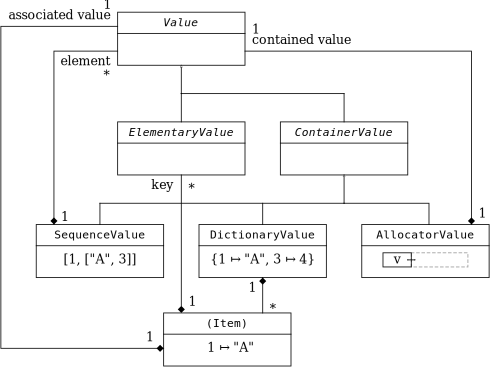
\includegraphics[scale=0.7]{classdiag_container}%
        \caption{Class hierarchy of container values.}
        \label{fig:class:ContainerValue}
    \end{quote}
\end{figure}


\subsubsection{\DborSequenceValue($v_1, \ldots, v_r$)}
%%%%%%%%%%%%%%%%%%%%%%%%%%%%%%%%%%%%%%%%%%%%%%%%%%%%%%
\hypertarget{sec:def:SequenceValue}{}

\paragraph{Representable objects}

A \DborSequenceValue{} can represent any sequence $v_1, \ldots, v_r$
of well-formed values (its elements) with the total size $\sum_{i = 1}^r \|v_i\| \in \IntegerInterval{0}{N + 23}$.

\paragraph{Representation}

A representable sequence $v_1, \ldots, v_r$ is represented as
\DborIntegerToken*($4$, $m$) {\Concat} $v_1 \Concat \cdots \Concat v_r$
with $m := \sum_{i = 1}^r \|v_i\|$.

\smallskip
\noindent
Examples:\nolinebreak
\begin{quote}
    \noindent
    \begin{tabular}{lll}
        \toprule
        Value & Representation \\
        \midrule
        \DborSequenceValue()
            & \ByteSequence{\DborFirstByteSequence{80}} \\
        \DborSequenceValue(\DborNoneValue, \DborIntegerValue($24$))
            & \ByteSequence{\DborFirstByteSequence{83},
                    \DborFirstByteNone{FF},
                    \DborFirstByteNumber{18}, \DborNextByte{00}} \\
        \bottomrule
    \end{tabular}
\end{quote}

A non-empty byte sequence \ByteSequence{b_1, \ldots, b_n} is a \emph{well-formed}
\DborSequenceValue{} if and only if it is \DborIntegerToken*($4$, $m$),
followed by well-formed values with a total size $m$.
The sequence is an \emph{ill-formed} \DborSequenceValue{} if and only if it is not a well-formed
\DborSequenceValue{} but $b_1$ is the first byte of an \DborIntegerToken*($4$, $m$).

\paragraph{Ambiguity, canonical value}

Whether there is more than one \DborSequenceValue{} representing the same object depends on its
elements.
The canonical value of \DborSequenceValue{}($v_1, \ldots, v_r$) is
\DborSequenceValue($v_1', \ldots, v_r'$)
where $v_i'$ is the canonical value of $v_i$ for all $i \in \IntegerInterval{1}{r}$.


\subsubsection{\DborDictionaryValue($k_1 \mapsto v_1, \ldots, k_r \mapsto v_r$)}
%%%%%%%%%%%%%%%%%%%%%%%%%%%%%%%%%%%%%%%%%%%%%%%%%%%%%%%%%%%%%%%%%%%%%%%%%%%%%%%%
\hypertarget{sec:def:DictionaryValue}{}

\paragraph{Representable objects}

A \DborDictionaryValue{} can represent any dictionary $k_1 \mapsto v_1, \ldots, k_r \mapsto v_r$ with
\begin{itemize}
    \item
    pairwise distinct, well-formed \emph{elementary values}%
    \footnote{
        Comparision of keys is an important operation and must be fast.
        When the keys must be compared efficiently and the fill bytes in \DborAllocatedValue*{} must be
        ignored; a container value that can contain an \DborAllocatedValue*{} must be processed in depth
        which makes such a comparison operation complex and slow.
        Disallowing container values makes the comparison operation simple and fast.
    }
    $k_i$ (its keys) and

    \item
    well-formed values $v_i$ (the values associated to $k_i$)

    \item
    with the total size $\sum_{i = 1}^r \big(\|k_i\| + \|v_i\|\big) \in \IntegerInterval{0}{N + 23}$ and

    \item
    $v_{i - 1} \prec v_{i}$ for all $i \in \IntegerInterval{2}{r}$.
\end{itemize}

${\prec}$ is the strict partial order on the set of byte sequences defined as follows:
$v_i \prec v_j$ if and only if they are different with the first different byte smaller in $v_i$ than
in $v_j$.

\paragraph{Representation}

A representable dictionary $k_1 \mapsto v_1, \ldots, k_r \mapsto v_r$ is represented as
\DborIntegerToken*($5$, $m$) {\Concat} $k_1 \Concat v_1 \Concat \cdots \Concat k_r \Concat v_r$
with $m := \sum_{i = 1}^r \big(\|k_i\| + \|v_i\|\big)$.

\smallskip
\noindent
Examples:\nolinebreak
\begin{quote}
    \noindent
    \begin{tabular}{lll}
        \toprule
        Value & Representation \\
        \midrule
        \DborDictionaryValue()
            & \ByteSequence{\DborFirstByteDictionary{90}} \\
        \DborDictionaryValue($\DborNoneValue \mapsto \DborIntegerValue($24$)$)
            & \ByteSequence{\DborFirstByteDictionary{93},
                    \DborFirstByteNone{FF},
                    \DborFirstByteNumber{18}, \DborNextByte{00}} \\
        \bottomrule
    \end{tabular}
\end{quote}

A non-empty byte sequence \ByteSequence{b_1, \ldots, b_n} is a \emph{well-formed}
\DborDictionaryValue{} if and only if
\begin{itemize}
    \item
    it is \DborIntegerToken*($5$, $m$),
    followed by an even number $2 r$ of well-formed values $k_1, v_1, \ldots, k_r, v_r$
    with total size $m$, and

    \item
    the $k_1, \ldots, k_r$ are all elementary values and

    \item
    $v_{i - 1} \prec v_{i}$ for all $i \in \IntegerInterval{2}{r}$.
\end{itemize}
The sequence is an \emph{ill-formed} \DborDictionaryValue{} if and only if it is not a well-formed
\DborDictionaryValue{} but $b_1$ is the first byte of an \DborIntegerToken*($5$, $m$).

\paragraph{Ambiguity, canonical value}

Whether there is more than one \DborDictionaryValue{} representing the same object depends on its
elements.
The canonical value of \DborDictionaryValue($k_1 \mapsto v_1, \ldots, k_r \mapsto v_r$) is
\DborDictionaryValue($k_1' \mapsto v_1', \ldots, k_r' \mapsto v_r'$)
where $k_i', v_i'$ are the canonical values of $k_i, v_i$ for all $i \in \IntegerInterval{1}{r}$.


\subsubsection{\DborAllocatedValue($m$, $v$)}
%%%%%%%%%%%%%%%%%%%%%%%%%%%%%%%%%%%%%%%%%%%%%
\hypertarget{sec:def:AllocatedValue}{}

\paragraph{Representable objects}

An \DborAllocatedValue{} can represent any object of fixed size $m \in \IntegerInterval{0}{N + 23}$
that contains exactly one well-formed value $v$ with $\|v\| \le m$.
This allows the definition of fixed offsets with a $v$ of variable size.

\paragraph{Representation}

A representable \DborAllocatedValue($m$, $v$) is represented as
\DborNaturalToken*($6$, $3$, $m$) {\Concat} $v \Concat \ByteSequence{f_{\|v\| + 1}, \ldots, f_m}$
with arbitrary fill bytes $f_{\|v\| + 1}, \ldots, f_m$.

\smallskip
\noindent
Examples:\nolinebreak
\begin{quote}
    \noindent
    \begin{tabular}{lll}
        \toprule
        Value & Representation \\
        \midrule
        \DborAllocatedValue(3, \DborIntegerValue(23))
            & \ByteSequence{\DborFirstByteAllocated{D8}, \DborNextByte{02},
                    \DborFirstByteNumber{17},
                    \DborNextByteFill{FF}, \DborNextByteFill{FF}} \\
        \DborAllocatedValue(3, \DborIntegerValue(24))
            & \ByteSequence{\DborFirstByteAllocated{D8}, \DborNextByte{02},
                    \DborFirstByteNumber{18}, \DborNextByte{00},
                    \DborNextByteFill{FF}} \\
        \bottomrule
    \end{tabular}
\end{quote}

A non-empty byte sequence \ByteSequence{b_1, \ldots, b_n} is a \emph{well-formed}
\DborAllocatedValue{} if and only if
it begins with \DborNaturalToken*($6$, $3$, $m$) for an appropriate $m$
and is followed by a well-formed value $v$ of size $\|v\| \le m$.
The sequence is an \emph{ill-formed} \DborAllocatedValue{} if and only if it is not a well-formed
\DborSequenceValue{} but $b_1$ is the first byte of a \DborNaturalToken*($6$, $3$, $m$).

\paragraph{Ambiguity, canonical value}

Whether there is more than one \DborAllocatedValue{} representing the same object depends on its
contained element.
The canonical value of \DborAllocatedValue($m$, $v$) is
\DborSequenceValue($m$, $v'$) where $v'$ is the canonical value of $i$
and all fill bytes $f_{\|v'\| + 1}, \ldots, f_m$ are $\HexNumber{FF}$.

    \section{Tokens}
%%%%%%%%%%%%%%%%
\label{sec:tokens}

\subsection{\DborSyntaxIdent{MinimalToken}($v$)}
%%%%%%%%%%%%%%%%%%%%%%%%%%%%%%%%%%%%%%%%%%%
\hypertarget{sec:def:MinimalToken}{}

A \DborSyntaxIdent{MinimalToken}($v$) for $v \in \SetOfIntegers \cap [0, 2^5)$
is the following byte:

\IncludeImageInPlace{MinimalToken}


\subsection{\DborSyntaxIdent{IntegerToken}($h$, $v$)}
%%%%%%%%%%%%%%%%%%%%%%%%%%%%%%%%%%%%%%%%%%%%%%
\hypertarget{sec:def:IntegerToken}{}

An \DborSyntaxIdent{IntegerToken}($h$, $v$) for $h \in \{0, 1, \ldots, 7\}$ and
$v \in \SetOfIntegers \cap [0, 24)$ is the following byte:

\IncludeImageInPlace{IntegerTokenA}

An \DborSyntaxIdent{IntegerToken}($h$, $v$) for $h \in \{0, 1, \ldots, 7\}$ and
$v \in \SetOfIntegers \cap [24, \sum_{k = 0}^8 2^{8k} + 23)$
is the following sequence of bytes:

\IncludeImageInPlace{IntegerTokenB}

Its $d_i \in \SetOfIntegers \cap [0, 2^8)$ are uniquely%
\footnote{%
    Since $(v - 23) \bmod 2^{8 j} = \sum_{i = 0}^{j - 1} (d_i + 1) 2^{8 i}$ for every $j$ with $0 < j \le k$,
    the $d_i$ can be calculated with increasing $i$.
}
defined by
\begin{equation}
    v = 23 + \sum_{i = 0}^k (d_i + 1) 2^{8 i}.
\end{equation}


\subsection{\DborSyntaxIdent{BinaryRationalToken}($p$, $o$, $s$, $M$, $E$)}
%%%%%%%%%%%%%%%%%%%%%%%%%%%%%%%%%%%%%%%%%%%%%%%%%%%%%%%%%%%%%%%%%%%%%%%%%%%
\hypertarget{sec:def:BinaryRationalToken}{}

A \DborSyntaxIdent{BinaryRationalToken}($p$, $o$, $s$, $M$, $E$) for
\begin{align*}
    p & \in \{4, 10, 16, 23, 30, 37, 44, 52\} \\
    o & \in \{0, 1\} \\
    s & \in \{0, 1\} \\
    M & \in \SetOfIntegers \cap [0, 2^p) \\
    E & \in \SetOfIntegers \cap [0, 2^r)
        \quad\text{with}\quad r := 8 k + 7 - p
        \quad\text{and}\quad k := \lfloor p / 7 \rfloor
\end{align*}%
and
\begin{align*}
    M = E = 0 \quad & \Rightarrow \quad p < 52 \\
    p < 52 \quad & \Rightarrow \quad o = 0
\end{align*}%
is the following sequence of bytes:

\IncludeImageInPlace{BinaryRationalToken}

It represents the value
\begin{equation}
    v = (-1)^s \cdot m \cdot 2^e
\end{equation}
with
\begin{align*}
    m & := 1 - o + M / 2^p \\
    e & := \max(E, o) - 2^{r-1} + 1.
\end{align*}

    % SPDX-License-Identifier: CC-BY-4.0
% DBOR specification - Dense Binary Object Representation
% Copyright (C) 2020 Daniel Lutz <dlu-ch@users.noreply.github.com>

\section{Implementation hints}
%%%%%%%%%%%%%%%%%%%%%%%%%%%%%%
\label{sec:implementation}

\subsection{Representation overview by first byte}
%%%%%%%%%%%%%%%%%%%%%%%%%%%%%%%%%%%%%%%%%%%%%%%%%%
\label{sec:implementation:representation_by_first_byte}

Values:\nolinebreak
\begin{quote}
    \noindent
    \newcolumntype{L}{>{$}l<{$}}% package 'array'
    \setlength\extrarowheight{0.7ex}
    \begin{tabular}{L v{0.5\textwidth} L}
        \toprule
        \text{First byte} & Value type & \text{Constraints} \\
        \midrule
        \DborFirstByteBin\DborNumberValueColour{000x\,xxxx}
            & \DborIntegerValue*($v$)
            & v \ge 0 \\
        \DborFirstByteBin\DborNumberValueColour{001x\,xxxx}
            & \DborIntegerValue*($v$)
            & v < 0 \\
        \DborFirstByteBin\DborStringValueColour{010x\,xxxx}
            & \DborByteStringValue*(\dots) \\
        \DborFirstByteBin\DborStringValueColour{011x\,xxxx}
            & \DborUtfEightStringValue*(\dots) \\
        \DborFirstByteBin\DborSequenceValueColour{100x\,xxxx}
            & \DborSequenceValue*(\dots) \\
        \DborFirstByteBin\DborDictionaryValueColour{101x\,xxxx}
            & \DborDictionaryValue*(\dots) \\
        \DborFirstByteBin\DborAllocatorValueColour{1100\,0xxx}
            & \DborAllocatorValue*(\dots) \\
        \DborFirstByteBin\DborNumberValueColour{1100\,1xxx}
            & \DborBinaryRationalValue*(\dots) \\
        \DborFirstByteBin\DborNumberValueColour{1101\,xxxx}
            & \DborDecimalRationalValue*(\dots, $e$)
            & |e| > 8 \\
        \DborFirstByteBin\DborNumberValueColour{1110\,xxxx}
            & \DborDecimalRationalValue*(\dots, $e$)
            & |e| \le 8 \\
        \BinNumber{1111\,0xxx}
            & - \\
        \BinNumber{1111\,10xx}
            & - \\
        \DborFirstByteBin\DborNumberlikeValueColour{1111\,1100}
            & \DborMinusZeroValue* \\
        \DborFirstByteBin\DborNumberlikeValueColour{1111\,1101}
            & \DborMinusInfinityValue* \\
        \DborFirstByteBin\DborNumberlikeValueColour{1111\,1110}
            & \DborInfinityValue* \\
        \DborFirstByteBin\DborNoneValueColour{1111\,1111}
            & \DborNoneValue* \\
        \bottomrule
    \end{tabular}
\end{quote}

\medskip
Tokens:\nolinebreak
\begin{quote}
    \noindent
    \newcolumntype{L}{>{$}l<{$}}% package 'array'
    \setlength\extrarowheight{0.7ex}
    \begin{tabular}{L v{0.5\textwidth} L}
        \toprule
        \text{First byte} & Token representation & \text{Constraints} \\
        \midrule
        \DborFirstByteBin\DborNumberValueColour{000x\,xxxx}
            & \DborIntegerToken*(0, $v$)
            & v \ge 0 \\
        \DborFirstByteBin\DborNumberValueColour{001x\,xxxx}
            & \DborIntegerToken*(1, $-v - 1$)
            & v < 0 \\
        \DborFirstByteBin\DborStringValueColour{010x\,xxxx}
            & \DborIntegerToken*($2$, $m$) {\Concat} \ByteSequence{b_1, \ldots, b_m} \\
        \DborFirstByteBin\DborStringValueColour{011x\,xxxx}
            & \DborIntegerToken*($3$, $m$) {\Concat} \ByteSequence{b_1, \ldots, b_m} \\
        \DborFirstByteBin\DborSequenceValueColour{100x\,xxxx}
            & \DborIntegerToken*($4$, $m$) {\Concat} $v_1 \Concat \cdots \Concat v_r$ \\
        \DborFirstByteBin\DborDictionaryValueColour{101x\,xxxx}
            & \DborIntegerToken*($5$, $m$) {\Concat} $k_1 \Concat v_1 \Concat \cdots \Concat k_r \Concat v_r$ \\
        \DborFirstByteBin\DborAllocatorValueColour{1100\,0xxx}
            & \DborNaturalToken*($6$, $0$, $m$) {\Concat} $v \Concat \ByteSequence{f_{\|v\| + 1}, \ldots, f_m}$ \\
        \DborFirstByteBin\DborNumberValueColour{1100\,1xxx}
            & \DborBinaryRationalToken*(\dots) \\
        \DborFirstByteBin\DborNumberValueColour{1101\,xxxx}
            & \DborPowerOfTenToken*($e$) {\Concat} \DborIntegerValue*(\dots)
            & |e| > 8 \\
        \DborFirstByteBin\DborNumberValueColour{1110\,xxxx}
            & \DborPowerOfTenToken*($e$) {\Concat} \DborIntegerValue*(\dots)
            & |e| \le 8 \\
        \BinNumber{1111\,0xxx}
            & \DborMinimalToken*($7$, $v$)
            & \HexNumber{10} \le v < \HexNumber{1B} \\
        \BinNumber{1111\,10xx}
            & \DborMinimalToken*($7$, $v$)
            & \HexNumber{1B} \le v < \HexNumber{1C} \\
        \DborFirstByteBin\DborNumberlikeValueColour{1111\,11xx}
            & \DborMinimalToken*($7$, $v$)
            & \HexNumber{1C} \le v < \HexNumber{1F} \\
        \DborFirstByteBin\DborNoneValueColour{1111\,1111}
            & \DborMinimalToken*($7$, $v$)
            & v = \HexNumber{1F} \\
        \bottomrule
    \end{tabular}
\end{quote}



\subsection{Check if canonical \DborBinaryRationalValue}
%%%%%%%%%%%%%%%%%%%%%%%%%%%%%%%%%%%%%%%%%%%%%%%%%%%%%%%%
\label{sec:implementation:BinaryRationalValue:canonical}

A byte sequence \ByteSequence{\HexNumber{D0} + k, d_0, \ldots, d_k} with
$k \in \IntegerInterval{0}{7}$ and $i := \lfloor \frac{k + 1}{4} \rfloor$
is a \DborBinaryRationalValue{} that is canonical if and only if
\begin{itemize}
    \item
    $k = 0$ or then

    \item
    $2^{2 - i} d_0 \bmod 2^8 \ne 0$ or then

    \item
    If $k < 7$:
    $(d_{ke} < 2 - i) \vee (d_{ke} > 4 + i)$
    with $d_{ke} := \lfloor d_k / 2^4 \rfloor \bmod 8$.

    If $k = 7$:
    $(d_k \BitAnd \HexNumber{7F} = 0) \wedge (d_{k - 1} \BitAnd \HexNumber{F0} = 0)
    \wedge (d_0 \BitOr \cdots \BitOr d_{k - 1} \ne 0)$
\end{itemize}


\subsection{Check if \DborIntegerValue{} represents multiple of 10}
%%%%%%%%%%%%%%%%%%%%%%%%%%%%%%%%%%%%%%%%%%%%%%%%%%%%%%%%%%%%%%%%%%%
\label{sec:implementation:IntegerValue:mod10}

An integer $v$ is an integer multiple of $10$ if and only if it is an integer multiple
of $2$ and of $5$.
Since $2^{8i} \bmod 2 = 0$ for $i \in \{0, 1, \ldots\}$
and $2^{8i} \bmod 5 = 1$ for $i \in \{1, 2, \ldots\}$,
a division of $v$ can be replaced by divisions of fewer bytes.

Example:
Let $\langle b, d_0, \ldots, d_k\rangle$ be \DborIntegerValue($v$) for $v \ge 24$.
Then
\begin{align*}
    v \bmod 2
        & = \big(23 + \sum_{i = 0}^k (d_i + 1) 2^{8 i}\big) \bmod 2
        = d_0 \bmod 2 \\
    v \bmod 5
        & = \big(23 + \sum_{i = 0}^k (d_i + 1) 2^{8 i}\big) \bmod 5
        = \big(\sum_{i = 0}^k (d_i \bmod 5) + k + 4\big) \bmod 5
\end{align*}


\end{document}
